\documentclass[10pt,twocolumn,letterpaper]{article}

\usepackage{cvpr}
\usepackage{times}
\usepackage{epsfig}
\usepackage{graphicx}
\usepackage{amsmath}
\usepackage{amssymb}
\usepackage[
natbib=true,
style=numeric,
sorting=none
]{biblatex}
\addbibresource{egbib.bib}

% Include other packages here, before hyperref.

% If you comment hyperref and then uncomment it, you should delete
% egpaper.aux before re-running latex.  (Or just hit 'q' on the first latex
% run, let it finish, and you should be clear).
\usepackage[breaklinks=true,bookmarks=false]{hyperref}

\cvprfinalcopy % *** Uncomment this line for the final submission

\def\cvprPaperID{****} % *** Enter the CVPR Paper ID here
\def\httilde{\mbox{\tt\raisebox{-.5ex}{\symbol{126}}}}

% Pages are numbered in submission mode, and unnumbered in camera-ready
%\ifcvprfinal\pagestyle{empty}\fi
\setcounter{page}{1}
\begin{document}

%%%%%%%%% TITLE
\title{Crowd counting on fixed camera images}

\author{Pierpaolo D'Odorico\\
{\tt\small pierpaolo.dodorico@studenti.unipd.it}
\and
Massimiliano Conte\\
{\tt\small massimiliano.conte@studenti.unipd.it}
}


\maketitle
%\thispagestyle{empty}
\begin{abstract}



In this work we compared different computer vision tecniques in order to estimate the number of people in a frame. The counting is performed on images captured from a fixed camera placed in a shopping mall. Some applications of this kind of counting on a static view are security and safety tasks, estimating the number of visitors on a mall for a/b testing purpose, planning spaces and services or verify compliance with covid-19 social distancing.

\end{abstract}

%%%%%%%%% BODY TEXT
\section{Introduction}

The crowd counting problem received a lot of attention in recent years, due to its direct connection with crowd control and public safety. For this reason many techniques were recently proposed.
Our idea is to compare two main tecniques in this fixed camera setting, one that is fast to implement and the other one more challenging, in order to verify if it is worth it to spend time for a more sophisticated solution. The first approach is to direcly estimate the number of people performing regression with a deep convolutional neural network, such as the VGG16 network \cite{simonyan2014very}. We chose this very deep network since it is easy to handle for our purposes, unlike more complex architectures that have, for example, skip layer connections, and also because it is the base for the second technique. The second approach performs an undirect estimate of the number of people. First it is estimated the density of people in the image, then starting from the obtained density map the count is inferred. This second approach represents the base idea for the state of the art methods in croud counting, where images could have a completely different number of people on  differents enviroment and perspective. After implementing the two approaches on our problem, we found that a simple regression based on neural networks could perform as good as density based approach, probably exploiting the fixed background.


%------------------------------------------------------------------------
\section{Related work}

We based our work on information contained in different papers about computer vision tasks and crowd counting. The first one is related to the base network of both approaches, the VGG16 net \cite{simonyan2014very}. In this paper the authors investigated the effect of a deeper (with respect to previous architectures) convolutional neural network on the classification accuracy in the
large-scale image recognition setting, specifically on the \textit{imageNet} dataset \cite{deng2009imagenet}. In this convolutional neural networks they used very small (3x3) convolution filters, which have shown a significant improvement on the prior state of the art configurations. They also pushed the depth to 16-19 weight layers (Fig.\ref{fig:vgg16}). Those convolutional filters learned during \textit{imageNet} classification task can be useful in our application, giving a meaningful feature extraction for finding people in images.

\begin{figure}[h!]
  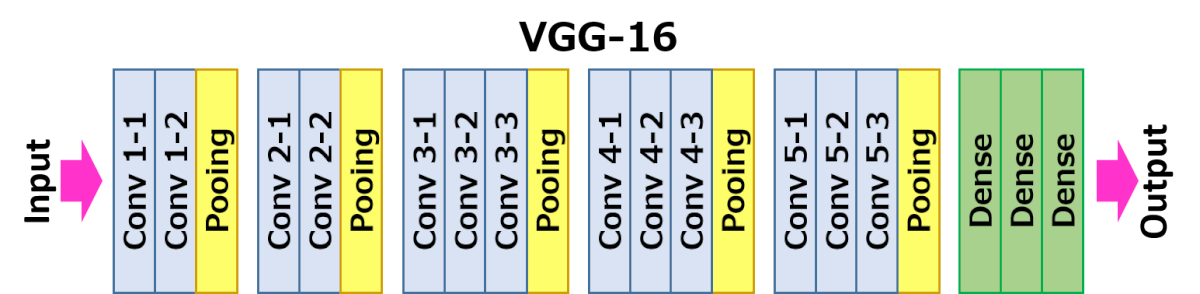
\includegraphics[width=\linewidth]{pics/vgg16.png}
  \caption{VGG16 deep CNN structure}
  \label{fig:vgg16}
\end{figure}

We relate also to two papers about density map crowd counting approach. In the first one \cite{zhang2016single} authors introduced a new large-scale crowd dataset named Shanghaitech. It contains nearly 1,200 images with around 330,000 accurately labeled heads. They also used Multi-column CNN for density map estimation (Fig.\ref{fig:densitymap}). We also relate to a more recent paper that simplifies the convolutional neural network of the previous work and achieves better results. This second paper about density map crowd couting approach \cite{li2018csrnet} uses a CSRNet architecture for capturing high-level features with
larger receptive fields and generating high-quality density maps without expanding network complexity. 

\begin{figure}[h!]
  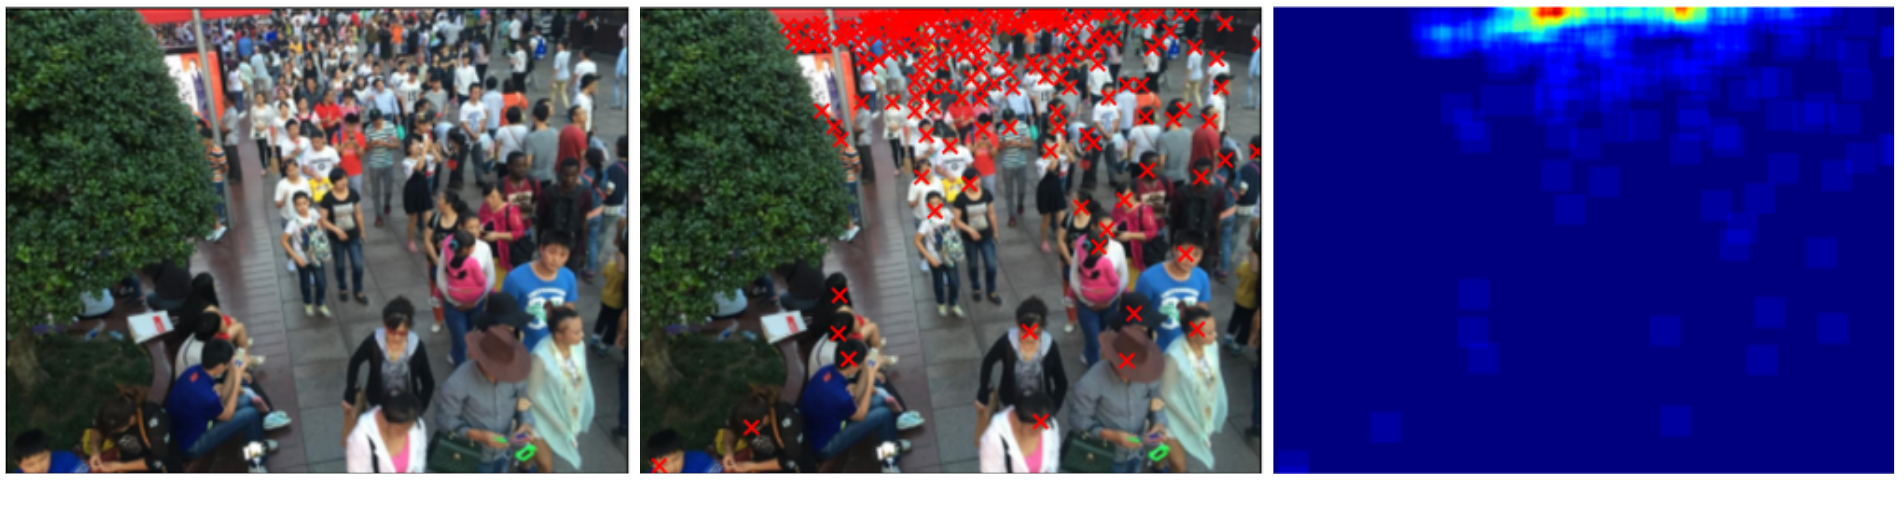
\includegraphics[width=\linewidth]{pics/densitymapapproach.png}
  \caption{Density map approach}
  \label{fig:densitymap}
\end{figure}



%------------------------------------------------------------------------
\section{Dataset}



\printbibliography

%{\small
%\bibliographystyle{ieee_fullname}
%\bibliography{egbib}
%}

\end{document}
